\section{Computational intelligence}

\subsection{Introduction}

Definitions to start the course 
\begin{itemize}
    \item \textbf{Problem} \ra Task to be solved automatically (find the maximum number in a list)
    \item \textbf{Algorithm} \ra Process to solve a problem, set of precise and not ambiguous actions that all together will allow us to reach the solution
    \item \textbf{Program} \ra Translation of an algorithm into a programming language
\end{itemize}

Motivation

\begin{itemize}
    \item In classical computational methods we start from a problem, and we have a human being that imagines an algorithm (problem-solving, it's creative and informal). Then software engineers will put the ideas into a computer in order to get a program (implementation, it's automatic and not creative). 
    \item We need computational intelligence because traditional methods in many cases fail, usually on the first step. We can have many problems where imaging solutions or algorithms it's either impossible or very hard for human being to imagine a solution. This is the case of \textbf{complex problems}
\end{itemize}


Some examples of complex problems
\begin{itemize}
    \item Categorization of clients
    \item Face recognition
    \item Find a new drug to cure a disease
    \item Driving a robot in a 3-D space 
\end{itemize}

Our idea is to give computers or informatic systems the ability to learn autonomously how to solve a problem. We define \textbf{learning} as improving something by means of experience. Those computers can also understand that the generated solution in not good enough, and so they should understand a better way to find the optimal solution. 

\vspace{10pt}

One of the most famous ways to improve those computers are bio-inspired algorithms. Like the \textbf{neural networks} (took inspiration from the brain), \textbf{evolutionary computation} (theory of evolution from Darwin, considering evolution as a sort of learning) where we have genetic algorithms, differential evolution or genetic programming, \textbf{swarm intelligence based algorithms} (system of animals are better at solve problems with respect to singular entities) like particle swarm optimization, \textbf{fuzzy systems} and \textbf{local search} like hill climbing simulated annealing.  

\vspace{10pt}

One category of complex problems are the so-called optimization problems. Even though they are complex they are easy to comprehend and to analyze.

Informally solving an optimization problem means to find the best solution(s) in a typically huge set of possible alternative solutions. We are able to find if something is a solution and to evaluate the quality of the solution with respect to the others. More formally an optimization problem is a pair of objects S and f where
\begin{itemize}
    \item S \ra set of all existing solutions (search space)
    \item f \ra function that evaluates the solutions (fitness or cost or quality function)
\end{itemize}

An optimization problem can be:

\[
\textbf{Maximization:} \quad \text{find } x^\ast \in S \text{ such that } 
f(x^\ast) \geq f(y) \quad \forall y \in S.
\]

\[
\textbf{Minimization:} \quad \text{find } x^\ast \in S \text{ such that } 
f(x^\ast) \leq f(y) \quad \forall y \in S.
\]

To solve this kind of problems we can use an optimization algorithm, a machine that is able to output multiple solutions (iterative machine). 

\vspace{10pt}

\textbf{No free lunch theorem} \ra the average performance of all optimization algorithms calculated on all existing optimization problems is the same. We care about the probability of finding the best solution and the time to reach it. We can't have one algorithm for every problem then we need to find a solution for every problem.


\subsection{Optimization algorithms}

\textbf{Optimization problem} \ra a pair (S, f) where

\begin{itemize}
    \item S is the set of all solutions (search space)
    \item f is the function (fitness function) where f : S \ra \begin{math}
        \mathbb{R} 
    \end{math}
\end{itemize}

An optimization problem can be:

\[
\textbf{Maximization:} \quad \text{find } x^\ast \in S \text{ such that } 
f(x^\ast) \geq f(y) \quad \forall y \in S.
\]

\[
\textbf{Minimization:} \quad \text{find } x^\ast \in S \text{ such that } 
f(x^\ast) \leq f(y) \quad \forall y \in S.
\]

x can be either a global optimum or a local one, we want to find the global(s) optima.

\vspace{10pt}

To find the solution we will use some optimization algorithm, by definition an optimization algorithm is an iterative method that at the end of each iteration returns a solution \begin{math}
    \in 
\end{math} S. One of the usual algorithm is \textbf{Random search}. 

As already seen we have the no free lunch theorem that stops us from finding a perfect solution. 

\vspace{10pt}
\textbf{No Free Lunch Theorem} \ra 
Let $A_1$ and $A_2$ be two optimization algorithms. 
When performance is averaged uniformly over all possible objective functions, 
$A_1$ and $A_2$ have identical expected performance.

\vspace{10pt}

The consequences of this theorem are that
\begin{enumerate}
    \item It is impossible to have an algorithm that is better than all the others and on all possible problems (no super algorithm can exist).
    \item Given a problem it can't exist an automatic method to find the best algorithm. Then we need to test, experiment and use our prior knowledge.
\end{enumerate}

\vspace{10pt}

Now we will see some algorithms. We start with \textbf{Hill climbing}. Before anything we need to clarify that we can't find every possible solution, so we need to use certain starting points.

\vspace{10pt}

\textbf{Neighborhood.}
Let $N : S \to 2^S$ be a neighborhood function that maps a solution 
$x \in S$ to a set of neighboring solutions $N(x) \subseteq S$.

Starting from an initial solution $x_0$ (typically chosen at random), 
the objective function is evaluated over $N(x_k)$, and the best 
neighbor is selected:
\[
x_{k+1} = \arg\min_{y \in N(x_k)} f(y)
\]
(for a minimization problem).

This process is repeated iteratively until a stopping criterion is met.

\vspace{10pt}

\textbf{Example}

\vspace{10pt}

\begin{itemize}
    \item S = {students in the room}
    \item f = student number 
    \item Maximization problem
    \item Neighborhood = the students around the selected student
\end{itemize}

\textbf{Local optimum} \ra given an optimization problem (S, f) a local optimum is a solution x such that $\forall y \in N(x), f(x)$ is better than $f(y)$. By definition hill climbing will return a local optimum with no guarantee that it will also be global. We can find the global optimum by expanding the radius or by trying more initialization

\vspace{10pt}

In pseudocode (general case)

\begin{enumerate}
    \item Initialize the current solution $x$ (typically at random).
    \item Repeat
    \begin{enumerate}[label=\theenumi.\arabic*]
        \item Generate a neighbor $y$ of $x$.
        \item If $f(y)$ is better than or equal to $f(x)$, set $x := y$.
    \end{enumerate}
    Until for all neighbors $y$ of $x$, $f(y)$ is worse than $f(x)$.
    \item Return $x$.
\end{enumerate}

In strict hill climbing we change the point only if the fitness is strictly better than the previous. With this setting we can have an infinite iteration between 2 equal points. We can set a timeout if we see the same points n times. 

Taboo search can help the search by using memory, avoid the already checked points. 

\vspace{10pt}

\textbf{Example}

\vspace{10pt}

\begin{itemize}
    \item $S = \{ i \in \mathbb{N} : 0 \le i \le 15 \}$
    \item  f(i) number of 1s in the binary code of i
    \item Maximization
    \item Neighborhood = i and j $\iff$ |i - j| = 1
\end{itemize}


We produce a plot

\begin{itemize}
    \item X \ra all solutions produced ordered by their neighborhood
    \item Y \ra all the fitness values
\end{itemize}

\begin{figure}[h!]
\centering
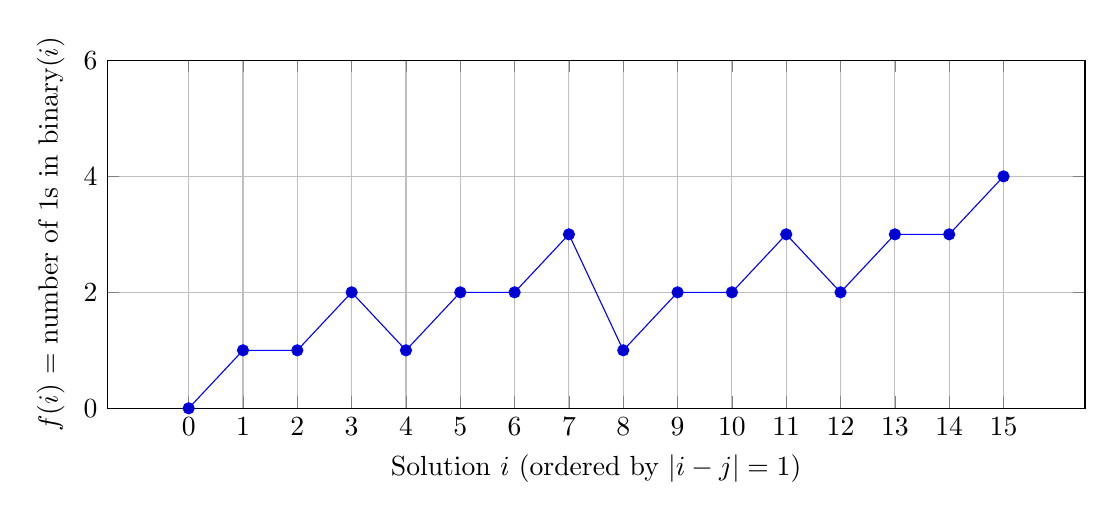
\begin{tikzpicture}
\begin{axis}[
    width=14cm,
    height=6cm,
    xlabel={Solution $i$ (ordered by $|i-j|=1$)},
    ylabel={$f(i)$ = number of 1s in binary$(i)$},
    xtick={0,...,15},
    ymin=0,
    ymax=6,
    grid=major
]

\addplot+[mark=*] coordinates {
(0,0)
(1,1)
(2,1)
(3,2)
(4,1)
(5,2)
(6,2)
(7,3)
(8,1)
(9,2)
(10,2)
(11,3)
(12,2)
(13,3)
(14,3)
(15,4)
};

\end{axis}
\end{tikzpicture}
\caption{Fitness landscape for $S=\{0,\dots,15\}$ with neighborhood $|i-j|=1$.}
\end{figure}

With the fitness landscape we can find the difficulty of the problem. A very smooth one is usually of a simple problem while a very oscillating one will be probably more difficult.


\subsection{Fitness landscape}

In the last class we saw what is a fitness landscape. The plot in the 2-D setting is obtained by plotting on the axis

\begin{itemize}
    \item Horizontal \ra All individual in the search space sorted according to the neighborhood
    \item Vertical \ra the fitness
\end{itemize}

Given an optimization problem (S, f) and a neighborhood N, a solution $x \in S$ is called a local optimum if $\forall y \in N(x)$ f(y) is worse than f(x). By construction hill climbing will return a local optimum with no guarantee that it will also be a global optimum.

\vspace{10pt} 

The fitness landscape gives a visual idea of how easy/hard is for an algorithm to solve the problem
\begin{itemize}
    \item Smooth \ra easy
    \item Rugged \ra hard
\end{itemize}

But in practice we can't draw the landscape because the search space is humongous, and the neighborhood is usually multidimensional.

\vspace{10pt}

Example
\begin{itemize}
    \item $S = \{ i \in \mathbb{N} | 0 \le i \le 15 \}$
    \item f(i) = $i^2$
    \item N = The solutions x and y are neighbors $\iff |x-y| = 1$
    \item Maximization
\end{itemize}

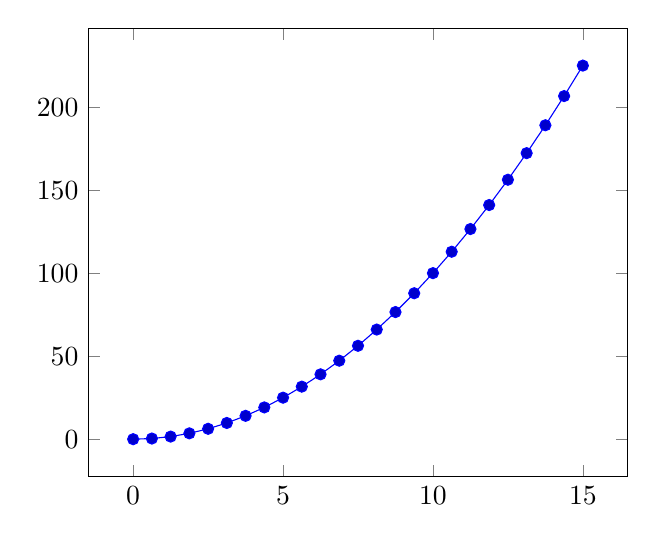
\begin{tikzpicture}
\begin{axis}[domain=0:15]
\addplot {x^2};
\end{axis}
\end{tikzpicture}

Here hill climbing will arrive at the global optimum.

\vspace{10pt}

If we want to look for the number of 1 in the binary code of i we can encounter problems and stay stuck in a local optimum without being able to find the global one. 
\vspace{10pt}

The definition of neighborhood is not fixed, we can define it in 2 ways.

\begin{itemize}
    \item N(x) \ra \{ $y \in s | d(x,y) \le k \}$ \ra distance based
    \item N(x) \ra \{ $y \in s | y = op(x) \}$ \ra action based
\end{itemize}


\begin{center}
\textbf{Example}
\end{center}

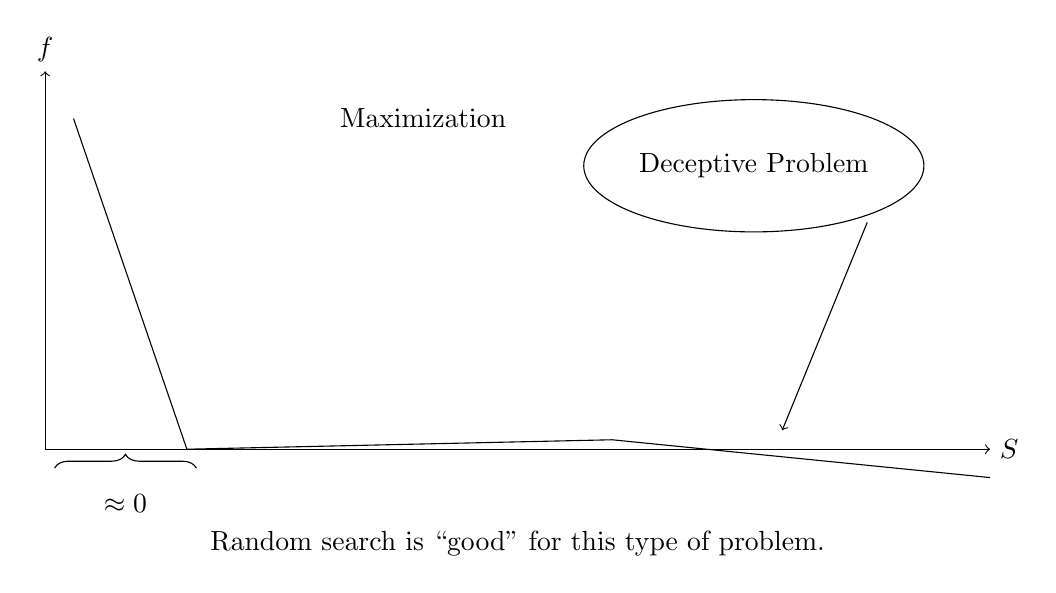
\begin{tikzpicture}[scale=1.2]

% axes
\draw[->] (0,0) -- (0,4) node[above] {$f$};
\draw[->] (0,0) -- (10,0) node[right] {$S$};

% deceptive peak near 0
\draw (0.3,3.5) -- (1.5,0);

% small mark around 0
\draw[decorate,decoration={brace,amplitude=5pt}]
(0.1,-0.2) -- (1.6,-0.2) node[midway,below=6pt] {$\approx 0$};

% almost flat line
\draw (1.5,0) -- (6,0.1) -- (8,-0.1) -- (10,-0.3);

% labels
\node at (4,3.5) {Maximization};

% deceptive problem bubble
\draw (7.5,3) ellipse (1.8 and 0.7);
\node at (7.5,3) {Deceptive Problem};

% arrow pointing to plateau
\draw[->] (8.7,2.4) -- (7.8,0.2);

% bottom text
\node at (5,-1) {Random search is ``good'' for this type of problem.};

\end{tikzpicture}

Hill climbing pros

\begin{itemize}
    \item Simple
    \item Efficient
    \item Versatile
\end{itemize}

Cons
\begin{itemize}
    \item Always stops on local optima
\end{itemize}

How to improve hill climbing

\begin{itemize}
    \item Parallel hill climbing
    \item Enlarge the neighborhood
    \item Give the possibility of worsening the fitness of the current solution (within a given probability)
\end{itemize}


\subsection{Annealing}

We now introduce the concept of annealing \ra an experiment aimed at finding the solid state of a material with the minimum level of energy.

\textbf{Metropolis algorithm}

\begin{enumerate}
    \item Consider the initial state of the material with energy $E_i$
    \item Alter the state to get a new energy $E_j$
    \item If $E_j \le E_i$ accept the new state and continue
    \item Else accept the state with probability $exp(-\frac{|E_i - E_j|}{K_B T})$
\end{enumerate}

Where 
\begin{itemize}
    \item T = Temperature
    \item $K_B$ = Boltzmann constant
\end{itemize}

\textbf{Simulated annealing}

\begin{itemize}
    \item Current solution = x
    \item Neighbor = y
\end{itemize}

\[
P(y) = \begin{cases}
    1 \text{ if f(y) better or equal than f(x)} \\
    exp(-\frac{|f(x) - f(y)}{C}) \text{ otherwise}
\end{cases}
\]

Where C is a control parameter

\subsection{Practical applications of Hill climbing}

Test case 1 \ra Given a set of possible investments (N), for each investment we know

\begin{itemize}
    \item Cost
    \item Estimated gain
\end{itemize}

We also know the budget of the client. What subset of the investments should our client do? 

Such that
\begin{itemize}
    \item The total cost is smaller or equal to the budget
    \item The profit is maximized
\end{itemize}


Using a numeric example

\begin{itemize}
    \item N = 10
    \item Costs = \{23, 31, 29, 44, 53, 38, 63, 85, 89, 82 \}
    \item Profits = \{92, 57, 49, 68, 60, 43, 67, 84, 87, 72 \}
    \item Budget = 165
\end{itemize}

\vspace{10pt}
Questions to answer
\begin{enumerate}
    \item What are the solutions ?
    \item How it is convenient to represent the solutions?
    \item What's the fitness?
    \item If the algorithm is neighborhood based, then what is the neighborhood?
\end{enumerate}

Golden rule \ra \textbf{DO NOT solve the problem}

Answers

\begin{enumerate}
    \item All the subsets of the set of investments
    \item As sequences of values, a string of bits of length N. The array will have a pair of  cost and profit. We use 0s and 1s to "1-hot encoding" them. 
    \item The sum for all the indexes where x is 1 of all the profits. $\sum\limits_{i:x[i]=1} p[i]$. We have a maximization problem. We only care about solutions that have a cost less than the budget. The fitness if this condition is not accepted we have -1 or 0 as fitness. Another way to define a non-good fitness is to use the negative sum of the costs such that the distance ourselves as much as possible from a bad solution. 
    \item The neighborhood is obtained here using the bit flip operator. 
\end{enumerate}


\vspace{10pt}

Test case 2 \ra Travel-sale-person: given N cities for which we know all the pairwise distances between themselves. Give one of these cities there is one specific one that is called home. We want the cyclic path that starts from home, visits all the cities once and only once and terminates at home using the shortest possible path.

\vspace{10pt}

We start from a matrix 

\begin{itemize}
    \item N = 5 \ra the matrix is 5x5
    \item Inside the matrix we have the costs/distances
\end{itemize}

Answers 

\begin{enumerate}
    \item Solutions \ra All cyclic paths starting and finishing in home and visiting all cities once. 
    \item Representation \ra An ordered string of the cities
    \item Fitness \ra the sum of the distances in the string
    \item Neighborhood \ra We can use a swapping operator
\end{enumerate}






